%% LyX 2.3.3 created this file.  For more info, see http://www.lyx.org/.
%% Do not edit unless you really know what you are doing.
\documentclass[twocolumn,english]{article}
\usepackage[T1]{fontenc}
\usepackage[latin9]{inputenc}
\usepackage{color}
\usepackage{babel}
\usepackage{float}
\usepackage{amsmath}
\usepackage{graphicx}
\usepackage[unicode=true]
 {hyperref}

\makeatletter
%%%%%%%%%%%%%%%%%%%%%%%%%%%%%% User specified LaTeX commands.
\usepackage{algorithm,algpseudocode}

\makeatother

\usepackage[style=numeric]{biblatex}
\addbibresource{project.bib}
\begin{document}
\title{Motion Planning for Autonomous Driving}
\author{Philippe Weingertner, Minnie Ho}
\maketitle

\section{Introduction}

\section{Related Work}

There is a rich litterature related to Motion Planning and a very
detailed survey of traditional methods is provided in \cite{7490340}.
Among the first 4 successful participants of DARPA Urban Challenge
in 2007, the approaches vary. The winner, CMU Boss vehicle used variational
techniques for local trajectory generation in a structured environment.
This was done in a 2 steps path-velocity decomposition. A first step
of path planning, using variational techniques, is performed and for
every candidate path, a combination of different velocity profiles
(constant, linear, linear ramp, trapezoidal) is applied : the combination
of a path and velocity profile defines a trajectory. In unstructured
environments (parking lots) or in error recovery situations a lattice
graph in 4-dimensional configuration space (position, orientation
and velocity) is searched with Anytime D{*} algorithm to find a collision-free
path. More details are provided in \cite{Ferguson2009MotionPI,article,5980223}.
The vehicle from Stanford used a search strategy coined Hybrid A{*}
that constructs a tree of motion primitives by recursively applying
a finite set of maneuvers. The search was guided by a carefully designed
heuristic. The vehicle arriving 3rd, Victor Tango from Virginia Tech,
constructs a graph discretization of possible maneuvers and searches
the graph with the A{*} algorithm. The vehicle arriving 4th, developed
by MIT used a variant of RRT algorithm with biased sampling. While
all these techniques differ, they fundamentally rely on a graph search
where nodes correspond to a configuration state and edges correspond
to elementary motion primitives. Although they provide solutions,
the runtime and state space can grow exponentially large. In this
context, the use of heuristic to guide the search is important. (\textbf{NB:
uncertainty is not properly considered here in these traditional MP
methods. It is like reasoning with the mean state vector provided
by sensor fusion output and ignoring the covariance matrix !})

More recently, Reinforcement Learning and Deep RL have been investigated
in the context of Autonomous Driving for Decision Making either at
the Behavioural Planning or Motion Planning level. In some research
papers from Volvo \cite{DBLP:journals/corr/abs-1803-10056} and BMW
\cite{inproceedings} , an RL agent is trained in simulation to take
decision at a higher tactical level: the decisions relate to a maneuver
selection, like lane change, rather than a low level acceleration
command. DQN is used to train an agent. But the problem with Reinforcement
Learning is that the utility is optimized in expectation. So even
if the reward is designed to avoid collisions, this will be optimized
in expectation: ultimately it is as if safety would be enforced with
soft constraints rather than hard constraints. Which is of course
not acceptable for a real vehicle. To solve this problem in \cite{inproceedings}
an additional safety check layer is added after the DQN agent to eventually
override the DQN agent decision if it is considered unsafe. Checking
a decision wrt to a specific criteria is simpler than designing a
decision making system that jointly optimizes efficiency, comfort
and safety objectives. With RL applied to AD we have to account for
additional safety checks. In \cite{DBLP:journals/corr/abs-1904-07189}
Deep RL is applied at the local planner level: the action space is
a set of longitudinal accelerations $\left\{ -4m/s^{2},-2m/s^{2},0m/s^{2},2m/s^{2}\right\} $
applied along a given path at a T-intersection. Safety is handled
in a different way here compared to previous BMW approach: the agent
is constrained to choose among a restricted set of safe actions per
state. So the safety is enforce before Deep RL. Ultimately car manufacters
may want to combine both types of safety checks: constraining the
action set per state before enabling an RL agent to make its own decision,
and checking again the final sequence of decisions proposed by the
RL agent.

Now the interesting topic is how to best combine traditional Motion
Planning with RL. What are the limitations of these techniques in
isolation and how to use the strengths of both approaches and circumvent
their weaknesses. Traditional motion planning relies heavily on tree
search and to enable real time solutions good heuristics are required.
Designing a good heuristic is hard. What if we could learn it ? By
training an agent with model free RL we can potentially end up with
an agent that performs pretty well most of the time and from time
to times fails miserably in a way that is hard to explain. The main
problems with model free RL are sample efficiency (we need a lot of
data), enforcing hard constraints and explainability (how can we explain
the decision taken by a RL agent which may become a problem for a
car manufacturer). While a model based planning method has the advantages
of explainability, do not rely on data and can deal in a more systematic
way with hard constraints. As demonstrated in \cite{DBLP:journals/corr/abs-1904-11483}
in simple situations RL methods have no benefit over rule based methods,
pure RL does not enable the agent to act in safer way. But when the
situation becomes much more complex with an increasing number of cars
and pedestrians, the benefits of Deep RL methods become clear.

In the gaming domain, chess and go, performances superior to human
performances have been achieved with AlphaGo Zero \cite{Silver2017MasteringTG}:
by combining planning with MCTS tree search and learning with RL.
A neural network biases the sampling towards the most relevant parts
of the search tree: a learnt policy-value function is used as a heuristic
during inference. While during training, MCTS is used to improve the
sample efficiency of RL training. Now there are a few major differences
between a game like chess or go and our initial Motion Planning problem.
In chess or go the state space is discrete and fully observable while
in AD the state space is continuous and partially observable. In terms
of action sets in both cases, we can deal with discrete action sets.
But another challenge is that self-play can not be used in the context
of Motion Planning. These challenges have been recently tackled in
different publications. The applicability of AlphaGo Zero to Autonomous
Driving has been studied in \cite{DBLP:journals/corr/abs-1905-02680,DBLP:journals/corr/abs-1905-12197,8814125}.

TODO: 
\begin{itemize}
\item analysis of the 3 most relevant papers
\item highlight what is specific to our use case
\end{itemize}

\section{Test Setup}

The problem statement is as follows. Given an ego vehicle (E) with
a given path of $(x,y)$ coordinates, find a set of acceleration decisions
$(a_{x},a_{y})$ at discrete time steps to enable E to avoid a set
of intersecting vehicles $\left\{ V\right\} .$

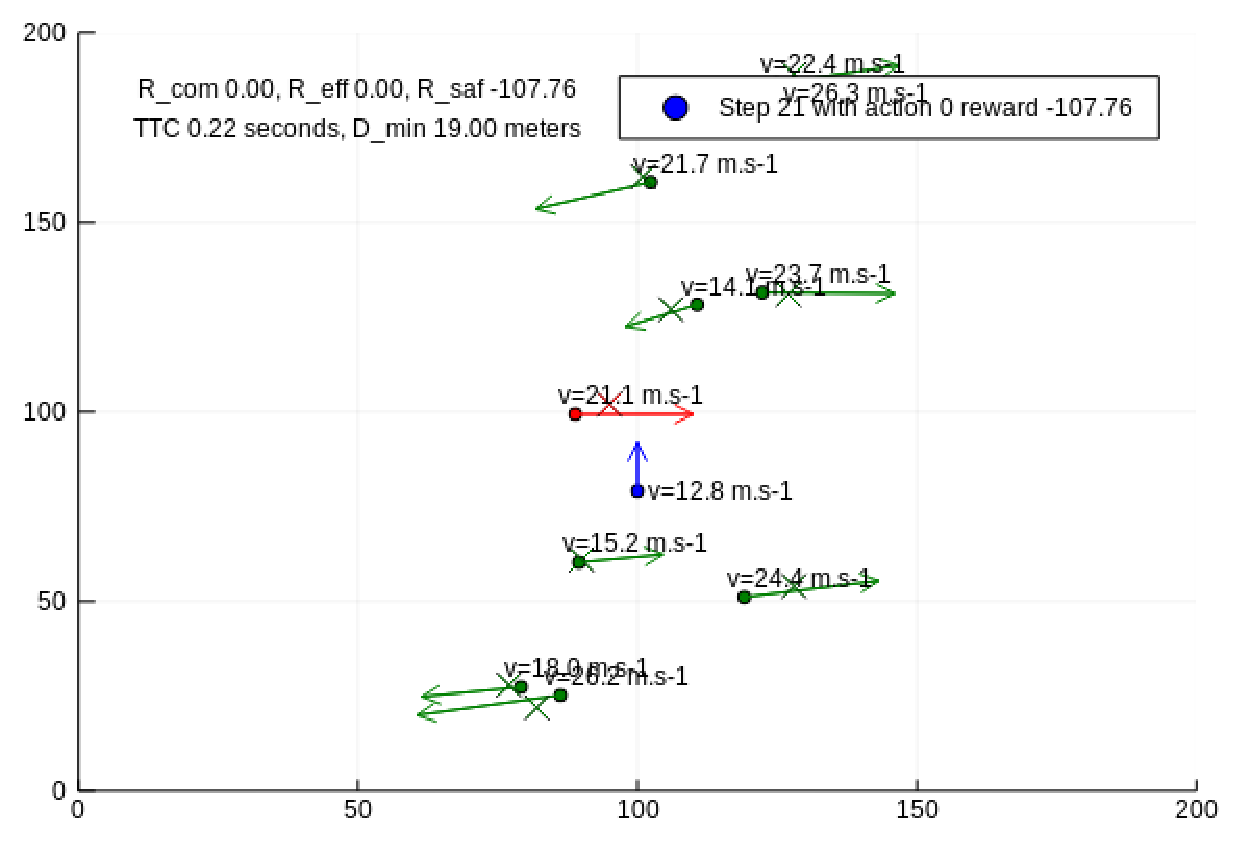
\includegraphics[scale=0.3]{img/ActV0}

The ego car in blue has to avoid 10 intersecting vehicles to reach
a goal point. The position and speed of intersecting vehicles is not
known precisely: the ground truth is represented via dots while the
position reported by the sensors is represented by crosses. A Time
To Collision based on ground truth information is displayed and if
there exist an intersecting car with a predicted TTC below 10 seconds
it is displayed in red. This test framework is a custom one we have
developped. We have a version of this test framework that is compatible
with open ai gym interfaces: so that any standard Deep RL setup, can
be directly used with this environment. Typically we intend to use
a DQN setup from \href{https://pytorch.org/tutorials/intermediate/reinforcement_q_learning.html}{pytorch.org}
initially tested on cartpole-v1 with our own Act-v1 environment. Our
simulation and test environment can be downloaded and installed from
\href{https://github.com/PhilippeW83440/CS221_Project/tree/master/gym-act}{gym-act}.

\section{Approach}

\subsection{MDP model}
\begin{itemize}
\item \textbf{State} (absolute coordinates): $S_{t}=\left\{ S_{i}^{t}\right\} _{i=0..11}=\left\{ \left(x,y,v_{x},v_{y}\right)_{\text{ego}},\left(x,y,v_{x},v_{y}\right)_{\text{obj}_{1..10}}\right\} $ 
\begin{itemize}
\item with $S_{i}^{t}=\left[x,y,v_{x},v_{y}\right]^{T}$ and $i\in\left[0,11\right]$
\end{itemize}
\end{itemize}
We use a relative and normalized $\in\left[-1,1\right]$ representation
of the state and account for the fact that the ego car drives along
the y-axis only (in a further simplified first version we could even
assume that the 10 other cars drive only along the x-axis, crossing
orthogonally to the ego car path):
\begin{itemize}
\item \textbf{State} (relative coordinates): $S_{t}=\left\{ S_{i}^{t}\right\} _{i=0..11}=\left\{ \left(\frac{y}{y^{max}},\frac{v_{y}}{v_{y}^{max}}\right)_{\text{ego}},\left(\frac{\Delta x}{\Delta x^{max}},\frac{\Delta y}{\Delta y^{max}},\frac{\Delta v_{x}}{\Delta v_{x}^{max}},\frac{\Delta v_{y}}{\Delta v_{y}^{max}}\right)_{\text{obj}_{1..10}}\right\} $
\item \textbf{Actions}: $a\in\left[-2\;ms^{-2},-1\;ms^{-2},0\;ms^{-2},1\;ms^{-2},2\;ms^{-2}\right]$
\begin{itemize}
\item for ego vehicle we choose an acceleration along y-axis
\end{itemize}
\item \textbf{Transitions}: $T\left(s'\mid s,a\right)=P\left(S_{i}^{t+1}\mid S_{i}^{t},a\right)=\mathcal{N}\left(T_{s}S_{i}^{t}+T_{a}\begin{bmatrix}a_{x}\\
a_{y}
\end{bmatrix}\right)$ 
\begin{itemize}
\item Linear Gaussian dynamics with a Constant Velocity Model
\item $T_{s}=\begin{bmatrix}1 & 0 & \text{dt} & 0\\
0 & 1 & 0 & \text{dt}\\
0 & 0 & 1 & 0\\
0 & 0 & 0 & 1
\end{bmatrix},T_{a}=\begin{bmatrix}\frac{\text{dt}^{2}}{2} & 0\\
0 & \frac{\text{dt}^{2}}{2}\\
\text{dt} & 0\\
0 & \text{dt}
\end{bmatrix}$
\item $\begin{bmatrix}x^{t+1}\\
y^{t+1}\\
v_{x}^{t+1}\\
v_{y}^{t+1}
\end{bmatrix}=\begin{bmatrix}x^{t}+v_{x}^{t}\text{dt}\\
y^{t}+v_{y}^{t}\text{dt}\\
v_{x}^{t}\\
v_{y}^{t}
\end{bmatrix}+\begin{bmatrix}a_{x}\frac{\text{dt}^{2}}{2}\\
a_{y}\frac{\text{dt}^{2}}{2}\\
a_{x}\text{dt}\\
a_{y}\text{dt}
\end{bmatrix}+\begin{bmatrix}\mathcal{\sigma}_{x}\\
\sigma_{y}\\
\sigma_{v_{x}}\\
\sigma_{v_{y}}
\end{bmatrix}$
\end{itemize}
\item \textbf{Reward}: efficiency + safety + comfort
\begin{itemize}
\item $R_{t}=-1-1000\times1\left[\text{d(ego,obj)}\leq10\right]-1\left[\left|a_{t}\right|=2\right]$
\end{itemize}
\end{itemize}

\subsection{Algo 1, MCTS tree search}

The MDP is solved online via MCTS tree search. Solving it offline
with Value Iteration is not an option as we are dealing with a huge
state space (it is actually a continuous state space and if we want
to discretize it it will be huge anyways). This planning method, RL
Model based, has a complexity that does not grow exponentially with
the horizon. 

{\scriptsize{}\begin{algorithmic}[1] 
\Function{SelectAction}{$s,d$} 
	\Loop
		\State \Call {Simulate}{$s,d,\pi_0$}
	\EndLoop
	\State \Return arg max$_a\text{ }Q(s,a)$
\EndFunction
\end{algorithmic}}{\scriptsize\par}

{\scriptsize{}\begin{algorithmic}[1] 

\Function{Simulate}{$s,d,\pi_0$} 
	\If {$d=0$}
		\State \Return $0$
	\EndIf

	\If {$s \notin T$} 
		\For {$a \in A(s)$}
			\State $(N(s,a),Q(s,a)) \gets (N_0(s,a),Q_0(s,a))$
		\EndFor
		\State $T=T \cup \{s\}$
		\State \Return \Call {Rollout}{$s,d,\pi_0$} 
	\EndIf

	\State $a \gets \text{arg max}_a\text{ }Q(s,a)+c\sqrt{\frac{logN(s)}{N(s,a)}}$ 
	\State $(s',r) \sim G(s,a)$
	\State $q \gets r+\lambda$ \Call {Simulate}{$s,d-1,\pi_0$}
	\State $N(s,a) \gets N(s,a)+1$
	\State $Q(s,a) \gets Q(s,a)+ \frac{q-Q(s,a)}{N(s,a)}$
	\State \Return $q$ 
\EndFunction

\end{algorithmic}}{\scriptsize\par}

{\scriptsize{}\begin{algorithmic}[1] 

\Function{Rollout}{$s,d,\pi_0$} 
	\If {$d=0$}
		\State \Return $0$
	\EndIf
	\State $a \sim \pi_0(s)$
	\State $(s',r) \sim G(s,a)$
	\State \Return $r+\lambda$ \Call {Rollout}{$s',d-1,\pi_0$}
\EndFunction
\end{algorithmic}}{\scriptsize\par}

TODO: add progressive widening to deal with a continuous state space.

\subsection{Algo 2, Approximate Q-learning}
\begin{itemize}
\item Model Free RL algorithm:
\begin{itemize}
\item $\hat{Q}_{\text{opt}}(s,a;\mathbf{w})=\mathbf{w}\cdot\phi(s,a)$
\item $\hat{V}_{\text{opt}}(s')=\underset{a'\in\text{Actions}(s')}{\max}\hat{Q}_{\text{opt}}(s',a')$
\item \textcolor{black}{$\text{Objective=}\left(\hat{Q}_{\text{opt}}(s,a;\mathbf{w})_{\text{pred}}-{\color{green}{\normalcolor \left(r+\gamma\hat{V}_{\text{opt}}(s')\right)_{\text{targ}}}}\right)^{2}$}
\item $\mathbf{w}\leftarrow\mathbf{w}-\eta\left[\hat{Q}_{\text{opt}}(s,a;\mathbf{w})_{\text{pred}}-{\color{green}{\normalcolor \left(r+\gamma\hat{V}_{\text{opt}}(s')\right)_{\text{targ}}}}\right]\phi(s,a)$ 
\end{itemize}
\item Features Extractor 1: $\phi(s,a)=\begin{bmatrix}s_{42\times1}\\
a_{1\times1}\\
s_{42\times1}^{2}\\
a_{1\times1}^{2}
\end{bmatrix}$ 

The state vector has 42 components (10 cars with 4 components each
and 2 components for the ego car), action is a single number. We use
quadratic components as well: as it is expected that the value of
a $(s,a)$ tuple will depend on distances computations. Typically
when computing Time To Collision, quadratic terms appear so we want
to provide these relevant features and figure out by learning the
weights associated to these features.
\item Features Extractor 2: $\phi(s,a)=\begin{bmatrix}s_{6\times1}\\
a_{1\times1}\\
s_{6\times1}^{2}\\
a_{1\times1}^{2}
\end{bmatrix}$ we just take into account ego car + closest car to work with a minimum
number of features. It may be easier to work with; to speed up learning.
\end{itemize}

\subsection{Algo 3, Deep Q-learning}

Model Free RL method. Our Neural Network has 42 neurons as input,
corresponding to the state vector, and 5 neurons as output. We will
use a Neural Network architecture slightly adapted from \cite{DBLP:journals/corr/abs-1803-10056}.
It is based on a CNN network as we want to have translational invariance
of the input. It should not matter to provide information about different
cars in one order or the other.
\begin{center}
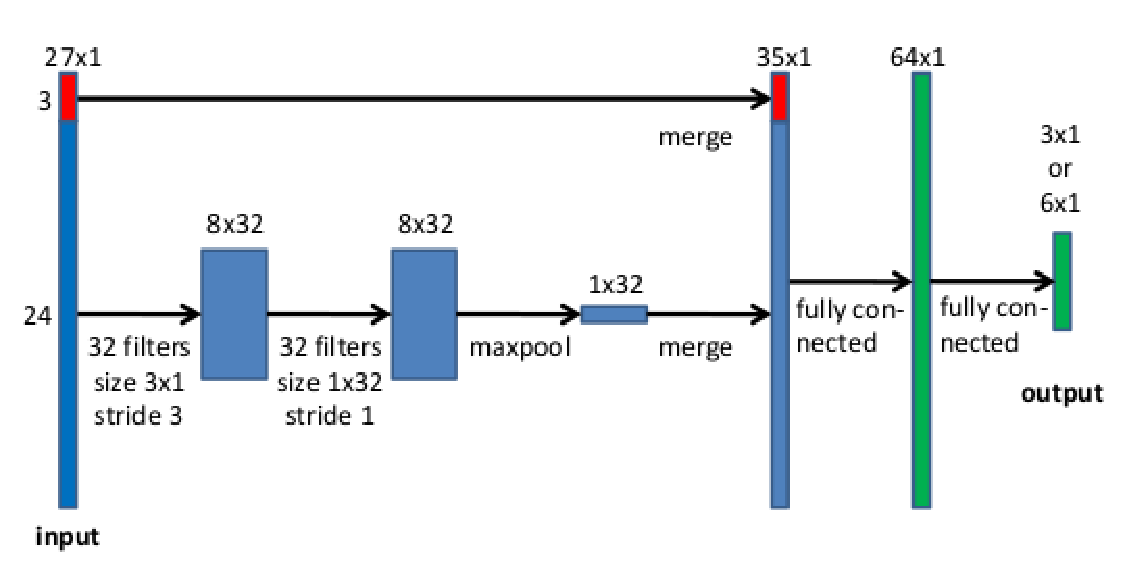
\includegraphics[scale=0.3]{img/CNN_for_DQN}
\par\end{center}

\subsection{Algo 4, MCTS tree search with a learned heuristic }

Combining Planning and Learning, Model Based and Model Free RL. TODO
post progress report.

We want to use our learned Q-network $\hat{Q}(s,a;\mathbf{w})$ via
approximate Q-learning or Deep Q-learning as a heuristic for MCTS
tree search: to expand the tree in the most promising areas and hence
come up faster with a good solution. A solution is considered good
as soon as it is estimated collision free; we may run further MCTS
tree searches up to some time limit, to find even better solutions:
faster or more comfortable. The reward takes into account safety,
comfort and efficiency. While there is a big penalty for collisions
of $-1000,$ at every time step we penalize the reward by $-1$ to
enforce efficiency and penalize every strong acceleration or deceleration,
when $\left|a\right|=2\quad ms^{-2}$, by -2 to encourage more comfortable
trajectories.

\section{Experimental Setup and Status}

The source code is available here: \href{https://github.com/PhilippeW83440/CS221_Project}{CS221 Project}
\begin{itemize}
\item Baseline: simple rule - reflex based. DONE
\item Oracle: assumes no uncertainty, UCS/A{*} tree search. DONE
\item Sequential Decision Making with Uncertainty => solve a MDP
\begin{itemize}
\item Planning with MCTS tree search. ON-GOING: MDP model implementation
+ our own MCTS algo implementation
\item Approximate Q-learning: leverage on CS221 hw4 blackjack setup + custom
Features Extractor + interface with our MDP model
\item Deep Q-learning: basically the pytorch DQN setup from \href{https://pytorch.org/tutorials/intermediate/reinforcement_q_learning.html}{pytorch.org}
customized with our proposed CNN network and interfaced with our own
gymai environment (gymai-act for Anti Collision Tests)
\item Combining Planning and Learning: we should have MCTS and Q-learning
working independently first ..
\end{itemize}
\end{itemize}
\nocite{*}
\printbibliography

\end{document}
